\documentclass[aps,twocolumn,letterpaper,twoside,nobalancelastpage,groupedaddress,amsmath,amssymb,floatfix,citeautoscript]{revtex4-1}
%\usepackage{geometry}       
%\geometry{letterpaper}     
%\usepackage[parfill]{parskip}    % Activate to begin paragraphs with an empty line rather than an indent
\usepackage{graphicx}
\usepackage{bm} %bold math symbols
\usepackage{times}
\usepackage{graphicx}             
%\usepackage{amssymb}
\usepackage[caption=false]{subfig}
%\usepackage{mathtools}
\usepackage{color}
\definecolor{darkred}{rgb}{0.6,0.,0.}
\definecolor{darkgreen}{rgb}{0.,0.5,0.}
\definecolor{darkblue}{rgb}{0.,0.,0.6}

\usepackage{framed}

%\usepackage[square,numbers,sort,merge]{natbib}
\usepackage[
breaklinks,
colorlinks=true,
linkcolor=darkred,
citecolor=darkgreen,
urlcolor=darkblue]{hyperref}
%\usepackage{doi}

% \DeclareMathOperator{\tr}{tr}
% \DeclareMathOperator{\erf}{Erf}

\DeclareGraphicsRule{.tif}{png}{.png}{`convert #1 `dirname #1`/`basename #1 .tif`.png}

\begin{document}


\def \Ns {\mathbb{N}}
\def \Rs {\mathbb{R}}
\def \Zs {\mathbb{Z}}
\def \Qs {\mathbb{Q}}
\def \Cs {\mathbb{C}}
\def \id {\mathbb{I}}

\def \bfq {{\bf q}}
\def \bfp {{\bf p}}
\def \bfx {{\bf x}}
\def \bfy {{\bf y}}
\def \bfz {{\bf z}}
\def \bfr {{\bf r}}
\def \bfk {{\bf k}}
\def \bfn {{\bf n}}
\def \bfb {{\bf b}}

%\def \hata {{a}}
%\def \hatadag {{a}^{\dagger}}

\def \hatq {\widehat{q}}
\def \hatp {\widehat{p}}
\def \hata {\widehat{a}}
\def \hatadag {\widehat{a}^{\dagger}}
%\def \hatb {\widehat{b}^\phantom{\dagger}}
%\def \hatbdag {\widehat{b}^{\dagger}}
\def \wtN {\widetilde{N}}

\def \ve {\varepsilon}
\def \vth {\vartheta}



\title{Hamiltonian quartic in momenta as the limit of a two-dimensional lattice model}
\author{David Bauer}
\email{dbauer@physics.ucla.edu}
\affiliation{Department of Physics and Astronomy, University of California at Los Angeles, 475 Portola Plaza, Los Angeles, California 90095, USA}

\author{Rahul Roy}
\affiliation{Department of Physics and Astronomy, University of California at Los Angeles, 475 Portola Plaza, Los Angeles, California 90095, USA}

\date{\today}
\begin{abstract}
Recent work on the quantum Hall effect (QHE) in lattice models and other systems with non-trivial geometry has opened the question of the extent to the stability of quantum Hall states is dependent on Landau levels. We construct a lattice model that has as its continuum limit a Hamiltonian with purely quartic momentum dependence, yielding single-particle states different from Landau levels in which one may study the QHE. We study the spectrum and band structure of the lattice Hamiltonian and its continuum limit, as well as the fractional quantum Hall effect (FQHE) of interacting particles in these bands. 
\end{abstract}

\pacs{0}

\maketitle

\section{Introduction}
\subsection{Background and motivation}

%%%%%%%%%% Reference
% The theoretical proposal and numerical observation of time-reversal breaking lattice models exhibiting fractional quantum Hall (FQH) phases, reviewed in Refs.~\onlinecite{Parameswaran:2013uf,Bergholtz:2013ue}, have sparked intense interest in these models (``fractional Chern insulators'' or FCIs) as a promising venue for observing FQH physics without the need for large external magnetic fields. The majority of our theoretical understanding of the the fractional quantum Hall effect (FQHE) has been framed in the context of continuum Landau levels, which occupy a special and highly atypical point in the space of all single-particle Hamiltonians. It is a matter of both theoretical and experimental interest to identify which of the special properties of Landau levels (LLs) are essential to the existence of the FQHE: as FCIs rapidly move towards experimental reality, one would like to easily identify experimental parameters where FQH-like phases are most robust.
%%%%%%%%

%[FQHE and landau levels]

Standard theories of the integer and fractional quantum Hall effects (IQHE and FQHE, respectively) are based on the single-particle Landau level orbits that arise in a 2-dimensional system in the presence of continuous Galilean and rotational symmetries. A prototypical example of such a theory is Laughlin's wavefunction for the $\nu = 1/m$ fractional quantum Hall states \cite{Laughlin:1983hk}, which employs the holomorphic structure of lowest Landau level (LLL) wavefunctions ultimately arising from these symmetries. Much recent literature has focused on the potential formation and properties of quantum Hall (QH) phases in the absence of such continuous symmetries. These developments lead to an understanding of the more universal aspects of QH systems, but also have the potential to elucidate features of QH states in lattice systems. 

%[FCIS]

 Time-reversal breaking lattice models with flattened bands may exhibit the FQHE when fractionally filled with interacting particles. Such models are known as fractional Chern insulators, and their study has led to recent interest in lattice FQH systems; recent work on these systems is reviewed in Refs \cite{Parameswaran:2013uf,Bergholtz:2013ue}. While these bands exhibit some properties of Landau levels essential to the appearance of the QHE, such as Chern number and flat energy dispersion, they are in general quite different from the Landau levels on which theories of the QHE are based. As yet, there is no general theory of FCI states at the level of generality of, for example, the Laughlin wavefunction. Other studies of the QHE in lattice systems and its relation to the topology of such systems include \textcite{Thouless:1982kq} and \textcite{Haldane:1988gh}. The QHE in the Hofstadter model specifically, especially in connection with atoms in optical lattice, is well-studied \cite{Sorensen:2005bt,Palmer:2006km,Hafezi:2007gz,Moller:2009ir,Kapit:2010ky,Sterdyniak:2012jo,Scaffidi:2014tg,Harper:2014vi}.

% Due to the topological nature of the FQH states, one expects 
 
%[Geometry and Hall viscosity]

In addition to explicitly studying the appearance of the QHE in lattice bands, one can consider the effects of the lattice that persist in the continuum limit, for example band mass anisotropy; this naturally leads to a geometrical description of the single particle orbits based on a non-Euclidean metric tensor \cite{Yang:2012ab,Haldane:2016aa}. The quantum Hall effect in the presence of non-trivial geometry -- that is, a non-Euclidean metric -- is connected with the theory of Hall viscosity, which is the linear response of a system to variations in the metric tensor\cite{Avron:1995aa,Cho:2014aa}. As an example of a system in which one cannot apply the usual, Euclidean geometry of Landau levels, \textcite{Haldane:2016aa} studied the continuum single-particle Hamiltonian containing quartic momentum terms and its connection to the IQHE and Hall viscosity.

%[Summary of our work]

In this work, we exhibit a square lattice model that in the continuum limit yields a Hamiltonian that to lowest order is quartic in momentum. We expect that generically a lattice tight-binding Hamiltonian will have a quadratic Hamiltonian as its continuum limit, possibly with rotationally asymmetric cross-terms. In this case, terms higher order in momentum that arise in taking the continuum limit can be studied perturbatively. Since quadratic momentum terms vanish exactly in our model, the quartic terms and their rotational symmetry breaking effects cannot be treated as perturbations. We explicitly show how such a Hamiltonian may arise as the continuum limit of a lattice model, exhibit the connections between the lattice and continuum models, and study the formation of the FQHE by interacting particles in the lattice bands. The Hamiltonian we study is a modification of the well-known Hofstadter Hamiltonian, and we now provide a brief introduction the Hofstadter model and discuss its continuum limit. We will then discuss some generalities of the continuum quartic Hamiltonian before moving to discuss our lattice model.

\subsection{The Hofstadter model in small flux}

We consider a two-dimensional tight binding model on a square lattice with perpendicular magnetic field $B=\partial_x A_y - \partial_y A_x$. Including just a nearest neighbor hopping term, the Hamiltonian for this system is the well-known Hofstadter Hamiltonian \cite{Harper:1955ft,Hofstadter:1976js}
\[
\label{eq-hof}
H = -t_1 \sum_{\langle i j \rangle} \left[ c_{\bm{r}_i}^{\dagger} c_{\bm{r}_j} \exp\left(i\theta_{\bm{r}_i,\bm{r}_j}\right)  + \text{h.c.} \right]
\]
where $i$,$j$ run over the sites of a square lattice and
\begin{equation*}
\theta_{\bm{r}_i,\bm{r}_j}= \frac{2\pi}{\phi_0}\int_{\bfr_{i}}^{\bfr_{j}} \! \bf{A} \cdot \text{d} \bm{\ell}.
\end{equation*}
In the Landau gauge, this Hamiltonian leads to the Harper eigenvalue equation
\[
\label{eq-harper}
-\psi_{n+1} - \psi_{n-1} -  2\cos(2 \pi n \phi/\phi_0 - k_{y}) \psi_{n} = \varepsilon \psi_{n}.
\]
Here we have set $t_1=1$. Following \cite{Harper:2014vi}, in the limit of small flux per plaquette, one can approximate this difference equation by a continuum differential equation
\begin{align*}
-\frac{1}{2}\frac{d^2\psi}{dx^2} - \cos\left(2\pi x \phi/\phi_0 \right)\psi(x) = \frac{\varepsilon}{2}\psi(x)
\end{align*}
and expand the cosine term to second order in $\phi$. Setting $\omega \equiv 2\pi\phi/\phi_0$, $\tilde{\varepsilon} \equiv \frac{\varepsilon +2}{2}$, this gives
\begin{align}
\label{eq:landau-hamiltonian}
-\frac{1}{2}\frac{d^2\psi}{dx^2} + \frac{1}{2}\omega^2 x^2~\psi(x) = \tilde{\varepsilon}\psi(x) ,
\end{align}
which we recognize as the Schr{\"o}dinger euqation for a harmonic oscillator as appears in the Landau level problem. We note that for small flux, the energy depends linearly on $\omega$ and thus $\phi$, as seen in the small-flux behavior of the Hofstadter ``butterfly'' spectral plot.

% \subsection{Summary}
% In the next section of this work, we will introduce the model of interest and study some of its properties, both in the lattice case and in the continuum limit. We introduce an interaction potential and diagonalize its projection to the lattice bands to study the formation of the fractional quantum Hall effect in these bands.

\subsection{Continuum quartic Hamiltonian}
\label{sec:continuum-hamiltonian}
We now discuss the continuum Hamiltonian with diagonal quartic momentum terms for an electron moving in 2D in the presence of a perpendicular magnetic field,
\begin{align}
\label{eq:quartic-continuum-hamiltonian}
H = \frac{1}{4m^3}\bm{\pi}^4,
\end{align}
where $\bm{\pi} = \mathbf{p}-e\mathbf{A} = (\pi_x,\pi_y)$  is the usual kinetic momentum operator and $m$ is constant with dimensions of mass; we set $m=1$ in what follows. The operators $\pi_x$ and $\pi_y$ satisfy the commutation relation $\left[\pi_x,\pi_y\right] = ieB \equiv i\omega$. As usual one can introduce ladder operators
\begin{align*}
a = \frac{1}{\sqrt{2\omega}}\left(\pi_x -i\pi_y\right),\\
a^{\dagger} = \frac{1}{\sqrt{2\omega}}\left(\pi_x + i \pi_y\right)
\end{align*}
such that $\left[a,a^{\dagger}\right]=1$. In terms of these operators,
\begin{align}
\label{eq:quartic-hamiltonian-ladder-ops}
H = \frac{\omega^2}{4}\left[3(a^{\dag}a)^2 + 3a^{\dag}a + \frac{3}{2} + \frac{1}{2}\left(a^{\dag~4} + a^4\right)\right].
\end{align}

By specializing to the Landau gauge $\mathbf{A} = (0,Bx)$, and noting the translation invariance in the $y$ direction, we can factor the eigenstates $\phi_{k_y}(x,y) = e^{ik_y y}\psi(x)$. The Schr{\"o}dinger equation for the stationary states of (\ref{eq:quartic-continuum-hamiltonian}) then reduces to
\[
\frac{1}{4}\frac{d^4\psi}{dx^4} + \frac{1}{4}\omega^4 \left(x-k_y\right)^4\psi(x) = \tilde{\varepsilon} \psi(x).
\]
We write the energy eigenvalue with a tilde to identify it as a continuum as opposed to lattice value. As in the usual Landau level problem, the spectrum is independent of $k_y$, as seen from the form (\ref{eq:quartic-hamiltonian-ladder-ops}) of the Hamiltonian, and we set $k_y=0$. A semi-classical argument applying the Bohr-Sommerfeld quantization condition lets us estimate the behavior of the energy eigenvalues in the high energy limit. We write the classical energy of this system
\[
E = \frac{p^4}{4} + \frac{1}{4}\omega^4 x^4,
\]
or
\[
p(x) = (4E-\omega^4 x^4)^{1/4}
\]
Imposing the Bohr-Sommerfeld condition
\[
\int \text{d}x~p(x) = n \in \mathbb{Z}
\]
yields
\begin{align*}
E \sim \omega^2 n^2,
\end{align*}
so that that for $n \gg 1$, the $n$-th eigenvalue of the quantum Hamiltonian $\tilde{\varepsilon}_n \sim n^2$.

To approximate the spectrum of this Hamiltonian, we write it in the form (\ref{eq:quartic-hamiltonian-ladder-ops}) and project to a finite, $M$-dimensional space of harmonic oscillator states $\{\left|{0}\right>,\left|{1}\right>,\ldots,\left|{M-1}\right>\}$. We then consider the eigenvalues and eigenvectors of this truncated matrix as approximations to the full, infinite dimensional Hamiltonian. Within this approximation scheme, the first two eigenvalues are $\varepsilon_0\approx0.349~\omega^2$, $\varepsilon_1\approx1.782~\omega^2$. In agreement with the above semi-classical argument, we find $\varepsilon_n\sim n^2$ asymptotically. The approximate ground state $\left|\tilde{0}\right>$ of the quartic Hamiltonian has nonzero overlaps only with states $\left|n\right>$ where $n\equiv0~(\text{mod}~ 4)$, for example $\left<0\right.\!\!\left|\tilde{0}\right> \approx 0.999$ and $\left<4\right.\!\!\left|\tilde{0}\right> \approx -0.042$, and these overlaps decrease exponentially for higher harmonic oscillator states. Details of the spatial eigenfunctions of this Hamiltonian are presented in \cite{Haldane:2016aa}.

\section{Lattice model}
We now modify the Hofstadter model Hamiltonian by adding additional hopping terms between sites separated by two lattice spacings in the $x$ or $y$ directions, shown schematically in Fig.~\ref{fig:hopping}. The full tight binding Hamiltonian is then 
\begin{align}
\label{eq:quartic-hofstadter-hamiltonian}
H = &-t_1 \sum\limits_{\langle i j \rangle} \left[ c_{\bm{r}_i}^{\dagger} c_{\bm{r}_j} \exp\left(i\theta_{\bm{r}_i,\bm{r}_j}\right)  + \text{h.c.} \right]\nonumber \\*
&-t_2 \sum\limits_{j,\bm{\gamma}} \left[ c_{\mathbf{r}_j + \bm{\gamma}}^{\dagger}~ c_{\mathbf{r}_j}\exp\left(i\theta_{\bm{r}_j,\bm{r}_{j} +\bm{\gamma}}\right)  + \text{h.c.} \right] 
\end{align}
where $i$,$j$ run over lattice sites and $\bm{\gamma}\in\{\pm 2\hat{\mathbf{x}},\pm 2\hat{\mathbf{y}}\}$. We will refer to this as the ``quartic Hofstadter'' Hamiltonian. This Hamiltonian leads to a modified version of the Harper equation 
\begin{align}
\label{eq-harper-2}
-&t_2\left(\psi_{n+2} + \psi_{n-2}\right) - t_1\left(\psi_{n+1} + \psi_{n-1}\right)\nonumber \\*
 &-2t_1\cos(2 \pi \phi n - k_{y})\psi_n\nonumber \\*
  &-2t_2\cos\left(4 \pi \phi n - 2k_{y}\right)\psi_n = \varepsilon \psi_{n}.
\end{align}

For rational flux per plaquette $\phi = p/q$, we can numerically diagonalize the Hamiltonian (\ref{eq:quartic-hofstadter-hamiltonian}) on a system with periodic boundary conditions to obtain energies $\varepsilon_n(\mathbf{k})$ and Bloch states $\left|n,\mathbf{k}\right>$. We plot the full energy spectrum at $\mathbf{k}=(0,0)$ for various rational $\phi$ in Fig.~\ref{fig:butterfly}, producing a modification of the well-known Hofstadter ``butterfly'' plot. Fig.~\ref{fig:ground-state} shows the $\mathbf{k}=(0,0)$ ground state eigenvalue shifted for comparison with the continuum energy. For $\phi=1/q$, we calculate the Berry curvature of the lowest band and numerically integrate it over the Brillouin zone to verify that the Chern number $c_1=1$

\begin{figure}[bht]
\centering
\includegraphics[width=2.4in]{/Users/dbauer/Physics/Manuscripts/quartic/quartic-hofstadter-hoppings-2.pdf}
\caption{\label{fig:hopping}Diagram of hopping terms in the quartic Hofstadter Hamiltonian (\ref{eq:quartic-hofstadter-hamiltonian}).}
\end{figure}

\begin{figure}[bht]
\centering
\includegraphics[width=3.0in]{/Users/dbauer/Physics/Manuscripts/quartic/quartic-butterfly.pdf}
\caption{\label{fig:butterfly} Energy eigenvalues of the quartic Hofstadter model for some rational values of flux per plaquette. This is the analog of the well-known ``Hofstadter butterfly'' for our model.}
\end{figure}

% \begin{figure}[bht]
% \subfloat{\includegraphics[width=1.45in]{/Users/dbauer/Physics/Manuscripts/quartic/quartic-hofstadter-hoppings-2.pdf}\label{fig:hopping}}
% \subfloat{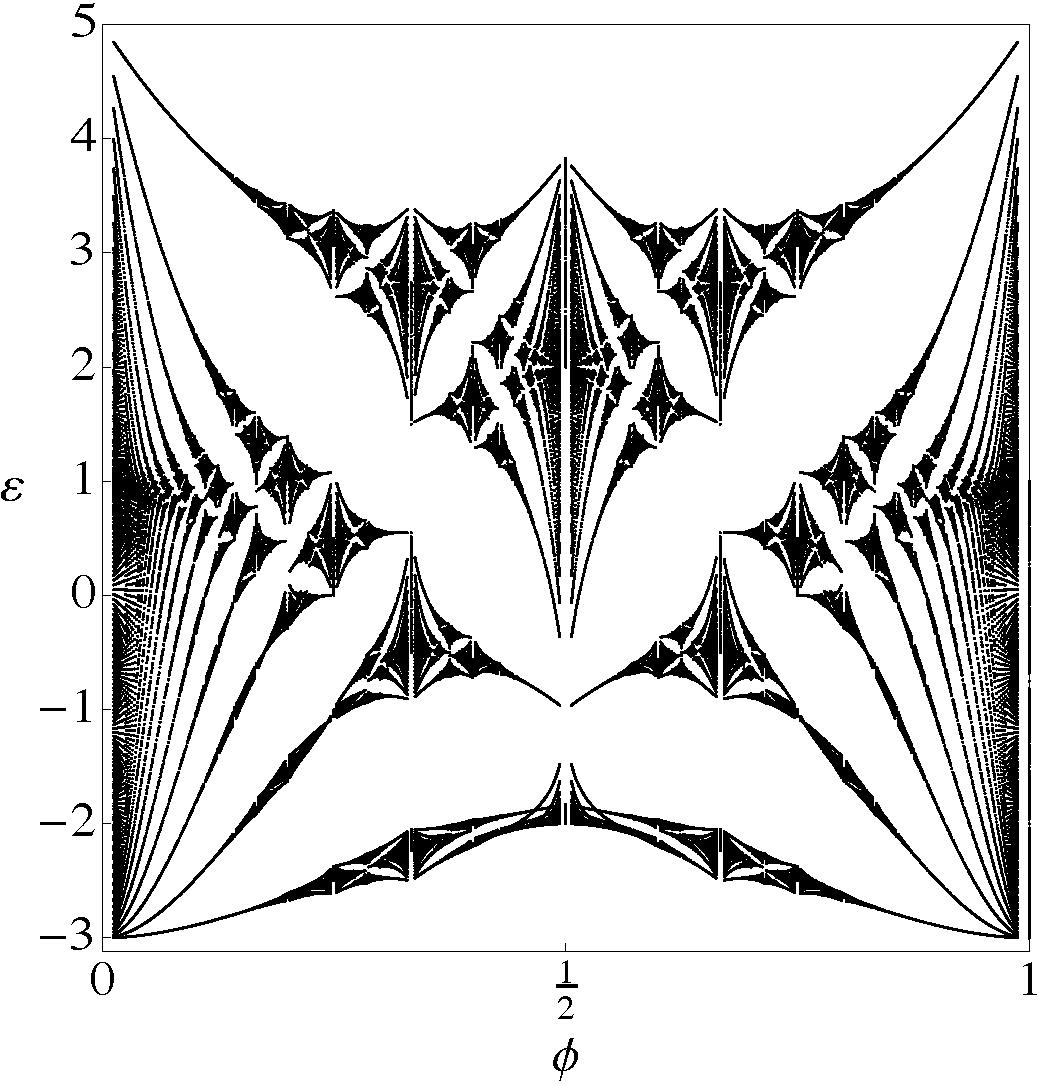
\includegraphics[width=1.45in]{/Users/dbauer/Physics/Manuscripts/quartic/quartic-butterfly-2.pdf}\label{fig:butterfly}}
% \caption{Test}
% \end{figure}


\begin{figure}[bht]
\centering
\includegraphics[width=3.0in]{/Users/dbauer/Physics/Manuscripts/quartic/lattice-eval-2.pdf}
\caption{\label{fig:ground-state} Energy in lowest quartic Hofstadter band at $\mathbf{k}=(0,0)$ for some rational values of flux per plaquette $\phi$. The red square shows the approximate lowest eigenvalue of the continuum Hamiltonian (\ref{eq:quartic-continuum-hamiltonian}).}
\end{figure}

As in the Hofstadter model, we can consider the small flux limit and find a corresponding continuum eigenvalue equation, approximating the finite difference
\[
\psi_{n+2} + \psi_{n-2} -4 \psi_{n+1} -4 \psi_{n-1} +6\psi_n \approx \frac{d^4\psi}{d x^4}.
\]
We then set the hopping strength so that $t_2 = -t_1/4$, and (\ref{eq-harper-2}) becomes
\begin{align}
&\frac{d^4\psi}{dx^4} - 8\cos(2 \pi \phi x) \psi(x)\nonumber \\*
 + &2\cos\left[2\left(2 \pi \phi x\right)\right]\psi(x) = \left(4\frac{\varepsilon}{t_1}+6\right) \psi(x),
\end{align}
setting $k_y=0$ as discussed. Expanding the cosine term and defining $\omega \equiv 2\pi\phi/\phi_0$, $\tilde{\varepsilon} \equiv \varepsilon/t_1 + 3$, the eigenvalue equation becomes
\[
\frac{1}{4}\frac{d^4\psi}{dx^4} + \frac{1}{4}\omega^4 x^4 \psi(x) = \tilde{\varepsilon} \psi(x),
\]
the Schr{\"o}dinger equation for the stationary states of (\ref{eq:quartic-continuum-hamiltonian}) in the Landau gauge.


\section{Interactions and FQH states}
To study the FQHE in this quartic model, we exactly diagonalize interactions projected to the lowest quartic Hofstadter band. We observed two different quantum Hall states, the $\nu = 1/2$ Laughlin state of bosons and the $\nu = 1/3$ Laughlin state of fermions. For each of these cases, we use $N_p = 8$ particles partially filling the lowest band on a lattice with periodic boundary conditions and topology of a torus. For the $\nu = 1/2$ case, we use a two-body repulsive delta function interaction, and place the particles on a lattice of $4 \times 4$ unit cells. We vary the flux per plaquette by increasing the size of each unit cell, using unit cells of dimension $m \times m$. For the $\nu = 1/3$ case, we use a lattice of $4 \times 6$ unit cells, with unit cell dimensions $3m \times 2m$.

For each many-body ground state, we observe signatures of relevant FQH topological order in the energy and entanglement spectra, including a quasi-degenerate ground state with gapped excitations, and a gap in the particle entanglement spectrum. The many-body gap as a function of flux per plaquette is plotted in Figs. \ref{fig:boson-gap} and \ref{fig:fermion-gap} for bosons and fermions, respectively.

%Many-body gaps as a function of flux per plaquette for Laughlin state of $N_{p}=8$ bosons at $\nu = 1/2$. (b). Laughlin state of $N_{p}=8$ fermions at $\nu = 1/3$. (c). Moore-Read state of $N_{p}=8$ bosons at $\nu = 1$.


\begin{figure}[bht]
\centering
\includegraphics[width=2.9in]{/Users/dbauer/Physics/Manuscripts/quartic/fqh-gap-boson.pdf}
\caption{\label{fig:boson-gap}Many-body gap as a function of flux per plaquette for Laughlin state of $N_{p}=8$ bosons at $\nu = 1/2$.}
\end{figure}

\begin{figure}[bht]
\centering
\includegraphics[width=2.9in]{/Users/dbauer/Physics/Manuscripts/quartic/fqh-gap-fermion.pdf}
\caption{\label{fig:fermion-gap}Many-body gaps as a function of flux per plaquette for Laughlin state of $N_{p}=8$ fermions at $\nu = 1/3$.}
\end{figure}


% \subsection{Band geometry of the quartic Hofstadter model}
As was done in \cite{Jackson:2015aa,Bauer:2016aa} for various lattice models, we can numerically study the geometry of the quartic Hofstadter model as a way to quantify deviations from lowest Landau level (LLL) behavior. The relationship between Chern band geometry and deviations from LLL physics was developed in \cite{Roy:2012vo} in terms of density operators projected to Chern bands. For $\phi=1/N$, the Chern number of each quartic Hofstadter band is 1. Deviations from the LLL can be measured by several band geometric quantities related to the Berry curvature and the Fubini-Study or quantum metric. In particular, inequalities relating the trace and determinant of the quantum metric to the Berry curvature are saturated in the LLL, and they are related to the closure of the algebra of projected density operators.

In \cite{Bauer:2016aa}, the Brillouin zone average of the ``trace inequality'' $\left<T\right>$ was shown to be related to the stability, especially in bands in which Berry curvature and quantum metric fluctuations can be neglected. In the Hofstadter model, $\left<T\right>$ vanishes in the small flux limit corresponding to the saturation of the inequality in the lowest Landau level. By contrast, we observe numerically that $\left<T\right>$ remains finite for the small flux limit quartic Hofstadter model, as is the case in, for example, higher Landau levels. We also note that the many-body gap of the quartic Hofstadter model appears correlated with $\left<T\right>$, as seen in Figs. \ref{fig:tr-gap} although the functional dependence differs from that in the Hofstadter model.

\begin{figure}[bht]
\centering
\includegraphics[width=2.9in]{/Users/dbauer/Physics/Manuscripts/quartic/gap-trace.png}
\caption{\label{fig:tr-gap}[Placeholder]}
\end{figure}

\section{Discussion}
In summary, we have exhibited a lattice model with a quartic Hamiltonian as its continuum limit, providing an example of continuum single-particle bands distinct from Landau levels that are capable of hosting the FQHE. 

The question of whether a generic picture of the stability of FCIs exists remains open, and one ideally would like to develop some means to calculate properties of the many-body FQH state from single particle bands. An analog of the Girvin-MacDonald-Platzman calculation of the many-body gap extended to Chern bands would be a useful tool.

Another interesting open question is what if any connection exists between the geometry of Chern bands and other geometric properties of QH states, for example the Hall viscosity.
[...]

\begin{acknowledgments}
D.B. thanks R. Snively and F. Harper for helpful conversations, and T.S. Jackson for collaboration during this work and for contributing code used in this paper.
\end{acknowledgments}

\bibliography{quartic-2}
% \bibliography{hofstadter-manual}

\end{document}


